\documentclass[compress,aspectratio=169]{beamer}

\usepackage{lmodern}
\usepackage{ujslide}              % UJ corporate style
\usepackage{graphicx}
\usepackage{url}
\usepackage[export]{adjustbox}
\usepackage{rotating}
\usepackage[natbib=true, bibstyle=numeric, citestyle=numeric]{biblatex}

% ---- Extra packages for tables and colour (used in the original report) ----
\usepackage{booktabs}
\usepackage{array}
\usepackage[table]{xcolor}
\usepackage{multirow}
\usepackage{tabularx}

% ---- Colour definitions from the report ----
\definecolor{taborange}{HTML}{DB5800}
\definecolor{statusdone}{HTML}{2E7D32}
\definecolor{statuspart}{HTML}{E65100}
\definecolor{statusplan}{HTML}{1565C0}

\newcommand{\Done}   {\textcolor{statusdone}{\textbf{Implemented}}}
\newcommand{\Partial}{\textcolor{statuspart}{\textbf{Partial}}}
\newcommand{\Planned}{\textcolor{statusplan}{\textbf{Planned}}}

% ---- Presentation metadata ----
\title[PDR \& Prototype]{Preliminary Design Review \& Prototype}
\subtitle{Multi-Author Writing Style Change Detection}
\author[T.P. Matlala]{Tshephang Phuti-A-Nkutu Matlala\\[0.5em]}
\institute[Academy of Computer Science and Software Engineering]{
    Academy of Computer Science and Software Engineering\\
    University of Johannesburg\\ South Africa}
\date{}
\logo{
\includegraphics[height=15mm]{ujlogo.pdf}}

\begin{document}

% ======================== TITLE SLIDE ========================
\begin{frame}
    \titlepage
\end{frame}

% ======================== OUTLINE ========================
\section*{Outline}
\begin{frame}{Outline}
    \tableofcontents
\end{frame}

% ======================== PRELIMINARY CONTEXT ========================
\section{About this Preliminary Design Review}
\begin{frame}{Preliminary Design Review Context}
    \begin{itemize}
        \item A Preliminary Design Review (PDR) examines the system’s design before detailed implementation begins.
        \item The design artefacts, test plan, and prototype presented here are \textbf{preliminary} – they will be refined as the project evolves.
        \item Test cases in this review are initial versions; they will be expanded, adapted, and re-prioritised during the development cycle.
        \item The prototype validates the core pipeline and interaction concepts, not the final feature set or performance.
    \end{itemize}
\end{frame}

% ======================== INTRODUCTION ========================
\section{Introduction}
\begin{frame}{What is Author Style Change Detection?}
    \begin{itemize}
        \item Detecting points in a document where the \textbf{writing style changes}.
        \item Implies the presence of \textbf{multiple authors}.
        \item Applications:
        \begin{itemize}
            \item Plagiarism and contract cheating detection.
            \item Forensic linguistics and authorship attribution.
            \item Analysis of collaborative writing (e.g., Wikipedia).
        \end{itemize}
        \item This project develops a \textbf{web-based tool} that automates detection using stylometric features and machine learning.
    \end{itemize}
\end{frame}

% ======================== PROBLEM STATEMENT ========================
\section{Problem Statement}
\begin{frame}{Problem Statement}
    \begin{block}{Challenges}
        \begin{itemize}
            \item Subtle stylistic differences between authors.
            \item Lack of large, annotated multi-author datasets.
            \item Need for \textbf{interpretable} results, not just black‑box predictions.
        \end{itemize}
    \end{block}
    \pause
    \begin{block}{Goal}
        Build a \textbf{proof‑of‑concept prototype} that:
        \begin{itemize}
            \item Extracts 31 stylometric features from sentence pairs.
            \item Trains a classifier to predict author switches.
            \item Provides confidence scores and explanatory features.
            \item Validates the feasibility of the processing pipeline and user interaction.
        \end{itemize}
    \end{block}
\end{frame}

% ======================== SYSTEM ARCHITECTURE ========================
\section{System Architecture}
\begin{frame}{Four‑Stage Pipeline}
    \begin{center}
        \textbf{Data} $\rightarrow$ \textbf{Features} $\rightarrow$ \textbf{Model} $\rightarrow$ \textbf{Evaluation}
    \end{center}
    \begin{columns}[T]
        \column{0.23\textwidth}
        \textbf{Data}\\
        \footnotesize
        Text upload, sentence segmentation, input validation.
        \column{0.23\textwidth}
        \textbf{Features}\\
        \footnotesize
        Stylometric feature extraction from each sentence pair.
        \column{0.23\textwidth}
        \textbf{Model}\\
        \footnotesize
        Classifier training (LR, SVM, k‑NN, MLP) and author‑switch prediction.
        \column{0.23\textwidth}
        \textbf{Evaluation}\\
        \footnotesize
        Cross‑validation, metrics, model comparison.
    \end{columns}
    \vspace{0.6cm}
    \begin{itemize}
        \item \textbf{Separation of concerns}: each package can be modified independently.
        \item Aligns with the conceptual class diagram (next slide).
    \end{itemize}
\end{frame}

\begin{frame}{Architecture Justification}
    The four-package decomposition provides:
    \begin{itemize}
        \item \textbf{Data} – isolates sentence segmentation and input validation changes.
        \item \textbf{Features} – allows new stylometric features without affecting other components.
        \item \textbf{Model} – enables independent replacement or extension of the classification algorithm.
        \item \textbf{Evaluation} – permits separate evolution of metrics and reporting.
    \end{itemize}
    \vspace{0.4cm}
    Benefits:
    \begin{itemize}
        \item Improved maintainability.
        \item Simplified unit and integration testing.
        \item Direct alignment with the domain model (conceptual class diagram).
    \end{itemize}
\end{frame}

\begin{frame}{Conceptual Class Diagram}
    \begin{center}
        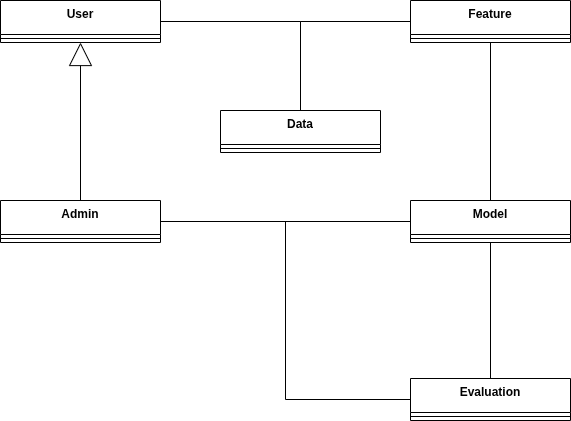
\includegraphics[width=\textwidth, height=0.6\textheight, keepaspectratio]{img/conceptual_class.pdf.png}
    \end{center}
    \footnotesize
    Core domain entities: \textbf{User}, \textbf{Admin}, \textbf{Data}, \textbf{Features}, \textbf{Model}, \textbf{Evaluation}.\\
    Implementation‑specific constructs (sentence buffers, prediction caches) are excluded – deferred to later design phases.
\end{frame}


% ======================== USE CASE TRACEABILITY ========================
\begin{frame}{Use Case Traceability}
    \centering
    \footnotesize
    \begin{tabular}{p{2.5cm} p{2.2cm} p{4.2cm} p{2.2cm}}
    \toprule
    \textbf{Use Case} & \textbf{Related FRs} & \textbf{Validating Tests} & \textbf{Status}\\
    \midrule
    UC1: Upload text for analysis & FR1--FR3 & UT-06--11, IT-01--03 & \Done\\
    UC2: View predictions & FR5--FR6 & IT-04--06, ST-01--02 & \Done\\
    UC3: Interpret confidence & FR7 & ST-01, UAT & \Partial\\
    UC4: Train model & FR8 & IT-07--08, ST-04 & \Done\\
    UC5: Compare model performance & FR9 & IT-11 & \Partial\\
    UC6: Login and authentication & Auth & UT-01--05 & \Partial\\
    \bottomrule
    \end{tabular}
\end{frame}

% ======================== PRELIMINARY TEST CASES (FULL) ========================
\section{Preliminary Test Cases}

\begin{frame}{Unit Test Cases – Authentication (UT-01 to UT-05)}
\centering
\footnotesize
\begin{tabularx}{\textwidth}{p{1.2cm} X X}
\toprule
\textbf{ID} & \textbf{Description} & \textbf{Expected Result}\\
\midrule
UT-01 & Username validation – valid & Username accepted\\
UT-02 & Username validation – invalid & Error message displayed\\
UT-03 & Password validation – correct & Login successful\\
UT-04 & Password validation – incorrect & Login rejected\\
UT-05 & Empty login fields & Validation error displayed\\
\bottomrule
\end{tabularx}
\end{frame}

\begin{frame}{Unit Test Cases – Document Processing (UT-06 to UT-11)}
\centering
\footnotesize
\begin{tabularx}{\textwidth}{p{1.2cm} X X}
\toprule
\textbf{ID} & \textbf{Description} & \textbf{Expected Result}\\
\midrule
UT-06 & Empty document upload & Upload rejected with warning\\
UT-07 & Valid text upload & Document processed successfully\\
UT-08 & Unsupported file format & Upload rejected with error message\\
UT-09 & Oversized document & Upload blocked\\
UT-10 & Sentence segmentation & Sentences split correctly\\
UT-11 & Single-sentence submission & Warning displayed\\
\bottomrule
\end{tabularx}
\end{frame}

\begin{frame}{Unit Test Cases – Feature Extraction (UT-12 to UT-16)}
\centering
\footnotesize
\begin{tabularx}{\textwidth}{p{1.2cm} X X}
\toprule
\textbf{ID} & \textbf{Description} & \textbf{Expected Result}\\
\midrule
UT-12 & Word count extraction & Count calculated correctly\\
UT-13 & Punctuation density & Density calculated correctly\\
UT-14 & Function-word ratio & Ratio computed correctly\\
UT-15 & Type-token ratio & Correct lexical richness value\\
UT-16 & Feature vector generation & Vector generated successfully\\
\bottomrule
\end{tabularx}
\end{frame}

\begin{frame}{Unit Test Cases – Prediction, Training \& Evaluation (UT-17 to UT-23)}
\centering
\footnotesize
\begin{tabularx}{\textwidth}{p{1.2cm} X X}
\toprule
\textbf{ID} & \textbf{Description} & \textbf{Expected Result}\\
\midrule
UT-17 & Prediction without model & Informative warning displayed\\
UT-18 & Prediction with trained model & Predictions generated successfully\\
UT-19 & Confidence-score generation & Confidence score displayed\\
UT-20 & Author-switch detection & Switch positions identified\\
UT-21 & Model training execution & Training completes successfully\\
UT-22 & Evaluation metrics & Precision, recall, F1 displayed\\
UT-23 & Model comparison & Comparison table displayed correctly\\
\bottomrule
\end{tabularx}
\end{frame}

\begin{frame}{Integration Test Cases (IT-01 to IT-11)}
\centering
\footnotesize
\begin{tabularx}{\textwidth}{p{1.2cm} X X}
\toprule
\textbf{ID} & \textbf{Description} & \textbf{Expected Result}\\
\midrule
IT-01 & Inspect endpoint – valid text & HTTP 200; sentence cards displayed\\
IT-02 & Inspect endpoint – file upload & HTTP 200; content parsed correctly\\
IT-03 & Inspect endpoint – empty body & Flash warning displayed\\
IT-04 & Predict endpoint – no model & Message: ``No model available''\\
IT-05 & Predict endpoint – with model & HTTP 200; predictions shown\\
IT-06 & Predict endpoint – fewer than 2 sentences & Flash warning displayed\\
IT-07 & Train endpoint – dataset missing & Flash error; log shows dataset error\\
IT-08 & Train endpoint – full pipeline & model.pkl created on disk\\
IT-09 & Explore endpoint – statistics & Statistics correct per difficulty level\\
IT-10 & Explore endpoint – both example types & Both columns displayed correctly\\
IT-11 & Model comparison endpoint & Side-by-side metrics displayed\\
\bottomrule
\end{tabularx}
\end{frame}

\begin{frame}{System Test Cases \& UAT}
\centering
\footnotesize
\begin{tabularx}{\textwidth}{p{1.2cm} X X}
\toprule
\textbf{ID} & \textbf{Description} & \textbf{Expected Result}\\
\midrule
ST-01 & End-to-end – two known switches & Both switches detected; top-3 features shown\\
ST-02 & End-to-end – single-author & Zero switches detected\\
ST-03 & Performance – 50 sentences & Processing completes in <10 seconds\\
ST-04 & End-to-end – train then predict & Model mode used; F1 displayed\\
\midrule
UAT & Proxy user workflow & Usability rating $\ge 4/5$\\
\bottomrule
\end{tabularx}
\vspace{0.3cm}
\raggedright\tiny
These preliminary test cases are subject to revision as the system evolves. All 38 entries are documented in the PDR document.
\end{frame}

% ======================== VALIDATION STRATEGY ========================

\begin{frame}{Validation Strategy}
\begin{center}
\textbf{Testing Pyramid}
\end{center}

\vspace{0.3cm}

\begin{enumerate}
    \item \textbf{Unit Testing}
    \begin{itemize}
        \item Validates feature extraction and document processing modules independently.
        \item Target coverage: $\geq 80\%$
    \end{itemize}
    
    \vspace{0.2cm}
    
    \item \textbf{Integration Testing}
    \begin{itemize}
        \item Verifies Flask routes and workflow interactions.
        \item Uses Flask test client for deterministic testing.
    \end{itemize}
    
    \vspace{0.2cm}
    
    \item \textbf{System Testing}
    \begin{itemize}
        \item Evaluates complete end-to-end user scenarios.
        \item Includes performance and prediction validation.
    \end{itemize}
    
    \vspace{0.2cm}
    
    \item \textbf{User Acceptance Testing}
    \begin{itemize}
        \item Proxy user performs upload-analyse-review workflow.
        \item Measures usability and interaction clarity.
    \end{itemize}
\end{enumerate}
\end{frame}

% ======================== KEY SYSTEM SCENARIOS ========================

\begin{frame}{Key System Scenarios}
\begin{block}{Scenario 1: Multi-Author Detection}
\begin{itemize}
\item User uploads a document containing multiple writing styles.
\item System extracts stylometric features between sentence pairs.
\item Classifier predicts author-switch positions with confidence scores.
\end{itemize}
\end{block}

\vspace{0.2cm}

\begin{block}{Scenario 2: Single-Author Validation}
    \begin{itemize}
        \item Document contains consistent writing style throughout.
        \item Expected result: zero author switches detected.
    \end{itemize}
\end{block}

\vspace{0.2cm}

\begin{block}{Scenario 3: Performance Requirement}
    \begin{itemize}
        \item 50-sentence document processed within interactive time.
        \item Acceptance target: under 10 seconds on reference hardware.
    \end{itemize}
\end{block}
\end{frame}

% ======================== PROTOTYPE ========================
\section{Prototype}
\begin{frame}{Prototype Overview}
    \begin{itemize}
        \item Implemented as a \textbf{Flask‑based web application} (Python).
        \item Technologies: Flask, NumPy, scikit-learn, HTML/CSS.
        \item Pages:
        \begin{itemize}
            \item \textbf{Home} – model status, quick‑start links.
            \item \textbf{Inspect} – upload text, view per‑sentence features.
            \item \textbf{Explore} – dataset statistics and examples.
            \item \textbf{Train} – classifier selection, training with live log.
            \item \textbf{Predict} – submit text, probability threshold, results.
        \end{itemize}
        \item Runs locally via \texttt{python app.py}; \texttt{http://localhost:5000}.
    \end{itemize}
\end{frame}

\begin{frame}{Functional Requirement Coverage}
    \centering
    \small
    \begin{tabular}{p{0.7cm} p{5.5cm} p{2.0cm} p{2.0cm}}
    \toprule
    \textbf{FR} & \textbf{Requirement} & \textbf{Prototype} & \textbf{Final}\\
    \midrule
    FR1  & Upload or paste text          & \Done   & \Done\\
    FR2  & Sentence segmentation         & \Done   & \Done\\
    FR3  & Input validation and errors   & \Done   & \Done\\
    FR4  & Stylometric feature extraction& \Done   & \Done\ (extra)\\
    FR5  & Pairwise feature differences  & \Done   & \Done\\
    FR6  & Author‑switch prediction      & \Done   & \Done\\
    FR7  & Confidence and top features   & \Partial& \Done\\
    FR8  & Admin model training          & \Done   & \Done\\
    FR9  & Model comparison              & \Partial& \Done\\
    Auth & User authentication           & \Partial& \Done\\
    \bottomrule
    \end{tabular}
    \vspace{0.3cm}
    
    \footnotesize\raggedright
    \textbf{Partial} items are implemented with limited functionality in the prototype and will be fully realised in the final system.
\end{frame}

\begin{frame}{Live Demo}
    \centering
    \Large
    Prototype Walkthrough\\
    \bigskip
    \normalsize
    The prototype will be demonstrated live, covering the Inspect, Train, and Predict workflows.\\
    \vspace{0.5cm}
    \footnotesize
    (Focusing mainly on Data Processing)
\end{frame}

% ======================== EVALUATION STRATEGY ========================
\section{Evaluation Strategy}
\begin{frame}{Test Plan – Objectives \& Levels}
    \begin{block}{Main objectives}
        \begin{enumerate}
            \item Validate all functional requirements against specifications.
            \item Classifier macro‑averaged F1 $>$ simple baseline on PAN 2026 held‑out set.
            \item Process 50‑sentence documents within interactive time (target: $<10$~s).
            \item Display top stylometric features associated with predicted switches.
            \item Graceful rejection of invalid/empty inputs.
            \item Correct authentication validation.
        \end{enumerate}
    \end{block}
    \pause
    \begin{block}{Test levels (pyramid)}
        \begin{description}
            \item[Unit] $\ge 80\%$ statement coverage; pytest with mocks.
            \item[Integration] Flask test client – upload, train, predict workflows.
            \item[System] End‑to‑end scenarios (multi‑author, single‑author, empty input).
            \item[UAT] Proxy user completes upload‑analyse‑review; $\ge 4/5$ usability rating.
        \end{description}
    \end{block}
\end{frame}

\begin{frame}{Test Strategy}
    \begin{itemize}
        \item \textbf{Approach:}
        \begin{itemize}
            \item White‑box: unit and integration tests (internal interfaces).
            \item Black‑box: system and acceptance tests (HTTP/UI interfaces).
        \end{itemize}
        \item \textbf{Framework:} \texttt{pytest} + \texttt{unittest.mock}; Flask test client for fast, deterministic HTTP simulation.
        \item \textbf{Test Data:}
        \begin{itemize}
            \item Unit tests: hand‑crafted sentences with known feature values.
            \item Integration / System: synthetic dataset with ground‑truth labels.
            \item Model evaluation: PAN~2026 held‑out test split.
        \end{itemize}
    \end{itemize}
\end{frame}

\begin{frame}{FR–Test Case Traceability}
    \centering
    \footnotesize
    \begin{tabular}{p{0.8cm} p{5.5cm} p{5.0cm}}
    \toprule
    \textbf{FR} & \textbf{Requirement} & \textbf{Covering Test Cases}\\
    \midrule
    FR1 & Upload or paste text      & UT-06--09, IT-01--02, ST-01\\
    FR2 & Sentence segmentation     & UT-10--11\\
    FR3 & Input validation          & UT-06, UT-08--09, UT-11, IT-03\\
    FR4 & Feature extraction        & UT-12--16\\
    FR5 & Pairwise differences      & UT-16\\
    FR6 & Author-switch prediction  & UT-17--20, IT-04--06, ST-01--02\\
    FR7 & Confidence and explanation& ST-01, UAT\\
    FR8 & Model training            & UT-21, IT-07--08, ST-04\\
    FR9 & Model comparison          & UT-23, IT-11\\
    Auth & Login authentication      & UT-01--05\\
    \bottomrule
    \end{tabular}
\end{frame}

\begin{frame}{Test Environment}
    \centering
    \footnotesize
    \begin{tabular}{p{3.5cm} p{7.5cm}}
    \toprule
    \textbf{Component} & \textbf{Details}\\
    \midrule
    Laptop Model & Acer Aspire A315-58\\
    Operating System & Fedora Linux 44 (Workstation Edition)\\
    Processor & 11th Gen Intel Core i3-1115G4\\
    Memory & 8 GB RAM\\
    Python Version & 3.10+\\
    Framework & Flask\\
    ML Library & scikit-learn\\
    Testing Framework & pytest\\
    Browsers & Chrome 124+, Firefox 125+\\
    \bottomrule
    \end{tabular}
\end{frame}

\begin{frame}{Risks and Contingency}
    \centering
    \footnotesize
    \begin{tabular}{p{3.5cm} p{1.5cm} p{6.0cm}}
    \toprule
    \textbf{Risk} & \textbf{Likelihood} & \textbf{Mitigation}\\
    \midrule
    PAN dataset unavailable & Medium & Use synthetic dataset as drop‑in replacement\\
    Classifier performance below baseline & Medium & Ablation study; add features if needed\\
    Time constraints limit UAT participants & High & One proxy instructor sufficient; structured walkthrough\\
    Training too slow for CI pipeline & Low & Mock classifier in integration tests; nightly full training\\
    \bottomrule
    \end{tabular}
\end{frame}

\begin{frame}{Processing a Document in a Short Time}
    \centering
    \begin{block}{Performance Target}
        The system shall process documents containing up to \textbf{50 sentences} within a time frame suitable for interactive use.
    \end{block}
    \vspace{0.3cm}
    \textbf{Specific goal (from acceptance criteria):}
    \begin{itemize}
        \item A fifty‑sentence document must be processed in \textbf{under ten seconds} on reference hardware.
    \end{itemize}
    \vspace{0.3cm}
    \footnotesize
    This requirement is validated by system test \texttt{ST-03} and ensures the tool remains practical for real‑time interactive analysis.
\end{frame}

\begin{frame}{Acceptance Criteria}
    The system is considered ready for the next development phase when:
    \begin{enumerate}
        \item All unit tests pass, with $\ge 80\%$ coverage in core processing modules.
        \item All documented integration scenarios execute without runtime errors.
        \item Preliminary classifier outperforms a simple baseline on the PAN 2026 held‑out test split.
        \item A fifty‑sentence document is processed in \textbf{$<10$ seconds} (performance requirement).
        \item UAT proxy user completes the upload‑analyse‑review workflow without assistance and gives a usability rating $\ge 4/5$ on a Likert scale.
    \end{enumerate}
\end{frame}

% ======================== PROTOTYPE DETAILS ========================
\begin{frame}{Prototype Implementation Details}
    \begin{itemize}
        \item \textbf{Inspect page (FR1–FR4):} text upload, sentence segmentation, 31 stylometric features per sentence, overview statistics, colour‑coded style‑distance bar.
        \item \textbf{Explore page:} dataset statistics and example display.
        \item \textbf{Train page (FR8):} classifier selection (Logistic Regression, SVM, k‑NN, MLP), cross‑validation, synchronous training with live log streaming.
        \item \textbf{Predict page (FR5–FR7):} text submission, probability threshold slider, ML‑based predictions when a model exists.
        \item \textbf{Results page:} held‑out F1, precision, recall, cross‑validation statistics.
        \item \textbf{Authentication (partial):} login form and session management; full validation deferred.
    \end{itemize}
    \vspace{0.3cm}
    \textbf{Known Limitations:}
    \begin{itemize}
        \item Random‑baseline predictor when no model is trained (UI exploration only).
        \item Synchronous training – will be moved to background task queue.
        \item Only \texttt{.txt} files (2 MB limit); PDF/DOCX support planned.
        \item Top feature computation uses raw difference vectors; permutation importance deferred.
    \end{itemize}
\end{frame}

% ======================== CONCLUSION ========================
\section{Conclusion}
\begin{frame}{Conclusion \& Future Work}
    \begin{block}{Key Achievements}
        \begin{itemize}
            \item Design review completed: modular architecture, conceptual class diagram, detailed test plan.
            \item Working proof‑of‑concept prototype validates the stylometric pipeline and user workflow.
            \item All core use cases (UC1–UC6) covered; FRs partially or fully implemented.
        \end{itemize}
    \end{block}
    \pause
    \begin{block}{Future Work (Final Implementation)}
        \begin{itemize}
            \item Asynchronous model training (background task queue).
            \item Support for PDF/DOCX uploads.
            \item Full user authentication and model comparison.
            \item Permutation‑based feature importance ranking.
        \end{itemize}
    \end{block}
\end{frame}

% ======================== REFERENCES ========================
\section{References}
\begin{frame}[allowframebreaks]{References}
    \tiny
    \begin{thebibliography}{99}
        \bibitem{myers2004art}
        G.~J. Myers, T.~Badgett, T.~M. Thomas, and C.~Sandler.
        \newblock {\em The Art of Software Testing}, 2nd ed.
        \newblock John Wiley \& Sons, 2004.

        \bibitem{zangerle_2026_19068843}
        E.~Zangerle, M.~Potthast, and B.~Stein.
        \newblock PAN 2026 shared task on multi‑author writing style change detection.
        \newblock In {\em Working Notes of CLEF}, 2026.
    \end{thebibliography}
\end{frame}

% ======================== CLOSING ========================
\section{Questions}
\begin{frame}{}
    \begin{center}
        \huge{Thank You}\\[1cm]
        \huge{Questions?}
    \end{center}
    \vspace{0.5cm}
    \begin{center}
        \url{223004635@student.uj.ac.za}
    \end{center}
\end{frame}

\end{document}